\documentclass{standalone}
\usepackage{tikz}
\usetikzlibrary{patterns, positioning}


\begin{document}
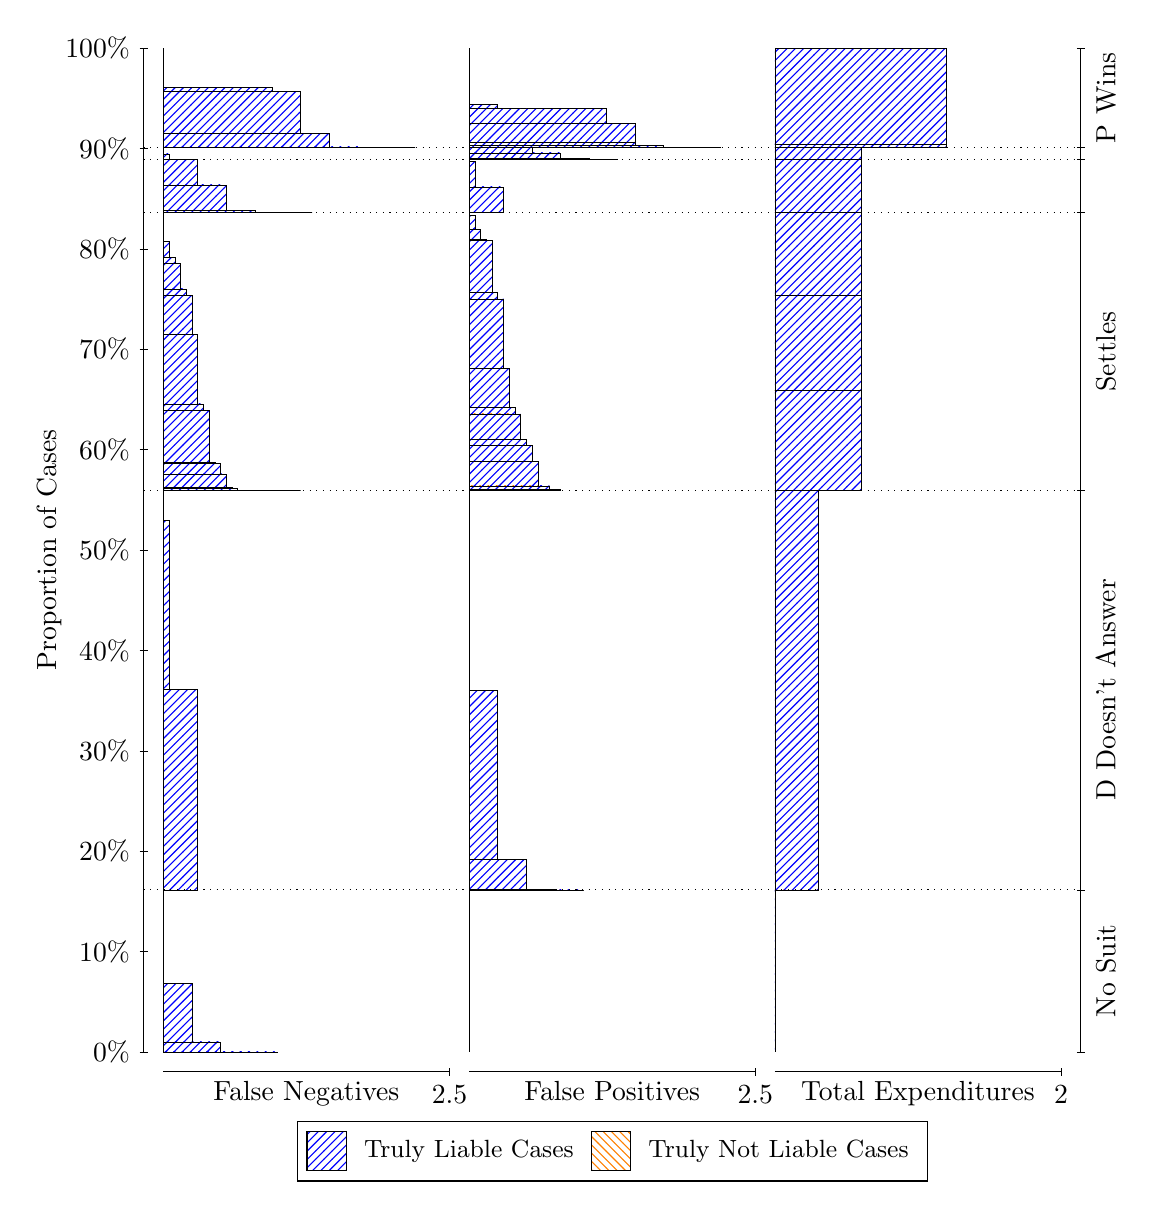
\begin{tikzpicture}
\draw[black, very thin] (1.5,1.75) -- (1.5,14.5);
\node[rotate=90, text=black, anchor=center] at (0.3, 8.125) {Proportion of Cases};
\draw[black, very thin] (1.45,1.75) -- (1.55,1.75);
\node[text=black, anchor=east] at (1.45, 1.75) {0\%};
\draw[black, very thin] (1.45,3.025) -- (1.55,3.025);
\node[text=black, anchor=east] at (1.45, 3.025) {10\%};
\draw[black, very thin] (1.45,4.3) -- (1.55,4.3);
\node[text=black, anchor=east] at (1.45, 4.3) {20\%};
\draw[black, very thin] (1.45,5.575) -- (1.55,5.575);
\node[text=black, anchor=east] at (1.45, 5.575) {30\%};
\draw[black, very thin] (1.45,6.85) -- (1.55,6.85);
\node[text=black, anchor=east] at (1.45, 6.85) {40\%};
\draw[black, very thin] (1.45,8.125) -- (1.55,8.125);
\node[text=black, anchor=east] at (1.45, 8.125) {50\%};
\draw[black, very thin] (1.45,9.4) -- (1.55,9.4);
\node[text=black, anchor=east] at (1.45, 9.4) {60\%};
\draw[black, very thin] (1.45,10.675) -- (1.55,10.675);
\node[text=black, anchor=east] at (1.45, 10.675) {70\%};
\draw[black, very thin] (1.45,11.95) -- (1.55,11.95);
\node[text=black, anchor=east] at (1.45, 11.95) {80\%};
\draw[black, very thin] (1.45,13.225) -- (1.55,13.225);
\node[text=black, anchor=east] at (1.45, 13.225) {90\%};
\draw[black, very thin] (1.45,14.5) -- (1.55,14.5);
\node[text=black, anchor=east] at (1.45, 14.5) {100\%};

\draw[black, very thin] (13.4,1.75) -- (13.4,14.5);
\draw[black, very thin] (13.35,1.75) -- (13.45,1.75);
\node[anchor=west] at (13.35, 1.75) {};
\draw[black, very thin] (13.35,3.8088) -- (13.45,3.8088);
\node[anchor=west] at (13.35, 3.8088) {};
\draw[black, very thin] (13.35,8.8854) -- (13.45,8.8854);
\node[anchor=west] at (13.35, 8.8854) {};
\draw[black, very thin] (13.35,12.41) -- (13.45,12.41);
\node[anchor=west] at (13.35, 12.41) {};
\draw[black, very thin] (13.35,13.089) -- (13.45,13.089);
\node[anchor=west] at (13.35, 13.089) {};
\draw[black, very thin] (13.35,13.236) -- (13.45,13.236);
\node[anchor=west] at (13.35, 13.236) {};
\draw[black, very thin] (13.35,14.5) -- (13.45,14.5);
\node[anchor=west] at (13.35, 14.5) {};

\draw[black, very thin, pattern color=blue, pattern=north east lines] (1.75,1.75) rectangle (3.2033,1.75);
\draw[black, very thin, pattern color=blue, pattern=north east lines] (1.75,1.75) rectangle (2.84,1.7511);
\draw[black, very thin, pattern color=blue, pattern=north east lines] (1.75,1.7511) rectangle (2.4767,1.8784);
\draw[black, very thin, pattern color=blue, pattern=north east lines] (1.75,1.8784) rectangle (2.1133,2.625);
\draw[black, very thin, pattern color=orange, pattern=north west lines] (1.75,2.625) rectangle (1.75,2.625);
\draw[black, very thin, pattern color=blue, pattern=north east lines] (1.75,2.625) rectangle (1.75,3.8088);
\draw[black, very thin, pattern color=blue, pattern=north east lines] (1.75,3.8088) rectangle (2.186,6.3546);
\draw[black, very thin, pattern color=blue, pattern=north east lines] (1.75,6.3546) rectangle (1.8227,8.4986);
\draw[black, very thin, pattern color=orange, pattern=north west lines] (1.75,8.4986) rectangle (1.75,8.4986);
\draw[black, very thin, pattern color=blue, pattern=north east lines] (1.75,8.4986) rectangle (1.75,8.8854);
\draw[black, very thin, pattern color=blue, pattern=north east lines] (1.75,8.8854) rectangle (3.494,8.8854);
\draw[black, very thin, pattern color=blue, pattern=north east lines] (1.75,8.8854) rectangle (3.3487,8.8854);
\draw[black, very thin, pattern color=blue, pattern=north east lines] (1.75,8.8854) rectangle (3.2033,8.8854);
\draw[black, very thin, pattern color=blue, pattern=north east lines] (1.75,8.8854) rectangle (3.1307,8.8854);
\draw[black, very thin, pattern color=blue, pattern=north east lines] (1.75,8.8854) rectangle (3.058,8.8854);
\draw[black, very thin, pattern color=blue, pattern=north east lines] (1.75,8.8854) rectangle (2.9853,8.8854);
\draw[black, very thin, pattern color=blue, pattern=north east lines] (1.75,8.8854) rectangle (2.9127,8.8858);
\draw[black, very thin, pattern color=blue, pattern=north east lines] (1.75,8.8858) rectangle (2.84,8.8866);
\draw[black, very thin, pattern color=blue, pattern=north east lines] (1.75,8.8866) rectangle (2.7673,8.8866);
\draw[black, very thin, pattern color=blue, pattern=north east lines] (1.75,8.8866) rectangle (2.6947,8.9151);
\draw[black, very thin, pattern color=blue, pattern=north east lines] (1.75,8.9151) rectangle (2.622,8.9185);
\draw[black, very thin, pattern color=blue, pattern=north east lines] (1.75,8.9185) rectangle (2.5493,9.0924);
\draw[black, very thin, pattern color=blue, pattern=north east lines] (1.75,9.0924) rectangle (2.4767,9.2234);
\draw[black, very thin, pattern color=blue, pattern=north east lines] (1.75,9.2234) rectangle (2.404,9.237);
\draw[black, very thin, pattern color=blue, pattern=north east lines] (1.75,9.237) rectangle (2.3313,9.9017);
\draw[black, very thin, pattern color=blue, pattern=north east lines] (1.75,9.9017) rectangle (2.2587,9.9808);
\draw[black, very thin, pattern color=blue, pattern=north east lines] (1.75,9.9808) rectangle (2.186,10.862);
\draw[black, very thin, pattern color=blue, pattern=north east lines] (1.75,10.862) rectangle (2.1133,11.362);
\draw[black, very thin, pattern color=blue, pattern=north east lines] (1.75,11.362) rectangle (2.0407,11.442);
\draw[black, very thin, pattern color=blue, pattern=north east lines] (1.75,11.442) rectangle (1.968,11.761);
\draw[black, very thin, pattern color=blue, pattern=north east lines] (1.75,11.761) rectangle (1.8953,11.84);
\draw[black, very thin, pattern color=blue, pattern=north east lines] (1.75,11.84) rectangle (1.8227,12.042);
\draw[black, very thin, pattern color=orange, pattern=north west lines] (1.75,12.042) rectangle (1.75,12.042);
\draw[black, very thin, pattern color=blue, pattern=north east lines] (1.75,12.042) rectangle (1.75,12.41);
\draw[black, very thin, pattern color=blue, pattern=north east lines] (1.75,12.41) rectangle (3.6393,12.41);
\draw[black, very thin, pattern color=blue, pattern=north east lines] (1.75,12.41) rectangle (3.276,12.41);
\draw[black, very thin, pattern color=blue, pattern=north east lines] (1.75,12.41) rectangle (2.9127,12.438);
\draw[black, very thin, pattern color=blue, pattern=north east lines] (1.75,12.438) rectangle (2.5493,12.762);
\draw[black, very thin, pattern color=blue, pattern=north east lines] (1.75,12.762) rectangle (2.186,13.089);
\draw[black, very thin, pattern color=orange, pattern=north west lines] (1.75,13.089) rectangle (1.75,13.089);
\draw[black, very thin, pattern color=blue, pattern=north east lines] (1.75,13.089) rectangle (2.186,13.09);
\draw[black, very thin, pattern color=blue, pattern=north east lines] (1.75,13.09) rectangle (1.8227,13.157);
\draw[black, very thin, pattern color=orange, pattern=north west lines] (1.75,13.157) rectangle (1.75,13.157);
\draw[black, very thin, pattern color=blue, pattern=north east lines] (1.75,13.157) rectangle (1.75,13.236);
\draw[black, very thin, pattern color=blue, pattern=north east lines] (1.75,13.236) rectangle (4.9473,13.236);
\draw[black, very thin, pattern color=blue, pattern=north east lines] (1.75,13.236) rectangle (4.584,13.236);
\draw[black, very thin, pattern color=blue, pattern=north east lines] (1.75,13.236) rectangle (4.2207,13.245);
\draw[black, very thin, pattern color=blue, pattern=north east lines] (1.75,13.245) rectangle (3.8573,13.419);
\draw[black, very thin, pattern color=blue, pattern=north east lines] (1.75,13.419) rectangle (3.494,13.948);
\draw[black, very thin, pattern color=blue, pattern=north east lines] (1.75,13.948) rectangle (3.1307,14.002);
\draw[black, very thin, pattern color=blue, pattern=north east lines] (1.75,14.002) rectangle (2.84,14.002);
\draw[black, very thin, pattern color=blue, pattern=north east lines] (1.75,14.002) rectangle (2.7673,14.002);
\draw[black, very thin, pattern color=blue, pattern=north east lines] (1.75,14.002) rectangle (2.4767,14.002);
\draw[black, very thin, pattern color=blue, pattern=north east lines] (1.75,14.002) rectangle (2.1133,14.004);
\draw[black, very thin, pattern color=orange, pattern=north west lines] (1.75,14.004) rectangle (1.75,14.004);
\draw[black, very thin, pattern color=blue, pattern=north east lines] (1.75,14.004) rectangle (1.75,14.5);
\draw[black, very thin, pattern color=orange, pattern=north west lines] (5.6333,1.75) rectangle (5.6333,1.75);
\draw[black, very thin, pattern color=blue, pattern=north east lines] (5.6333,1.75) rectangle (5.6333,3.8088);
\draw[black, very thin, pattern color=orange, pattern=north west lines] (5.6333,3.8088) rectangle (7.0867,3.8088);
\draw[black, very thin, pattern color=blue, pattern=north east lines] (5.6333,3.8088) rectangle (7.0867,3.8088);
\draw[black, very thin, pattern color=blue, pattern=north east lines] (5.6333,3.8088) rectangle (6.7233,3.8112);
\draw[black, very thin, pattern color=blue, pattern=north east lines] (5.6333,3.8112) rectangle (6.36,4.1956);
\draw[black, very thin, pattern color=blue, pattern=north east lines] (5.6333,4.1956) rectangle (5.9967,6.3396);
\draw[black, very thin, pattern color=blue, pattern=north east lines] (5.6333,6.3396) rectangle (5.6333,8.8854);
\draw[black, very thin, pattern color=orange, pattern=north west lines] (5.6333,8.8854) rectangle (6.796,8.8854);
\draw[black, very thin, pattern color=blue, pattern=north east lines] (5.6333,8.8854) rectangle (6.796,8.8991);
\draw[black, very thin, pattern color=orange, pattern=north west lines] (5.6333,8.8991) rectangle (6.6507,8.8991);
\draw[black, very thin, pattern color=blue, pattern=north east lines] (5.6333,8.8991) rectangle (6.6507,8.94);
\draw[black, very thin, pattern color=orange, pattern=north west lines] (5.6333,8.94) rectangle (6.5053,8.94);
\draw[black, very thin, pattern color=blue, pattern=north east lines] (5.6333,8.94) rectangle (6.5053,9.2538);
\draw[black, very thin, pattern color=blue, pattern=north east lines] (5.6333,9.2538) rectangle (6.4327,9.4553);
\draw[black, very thin, pattern color=orange, pattern=north west lines] (5.6333,9.4553) rectangle (6.36,9.4553);
\draw[black, very thin, pattern color=blue, pattern=north east lines] (5.6333,9.4553) rectangle (6.36,9.5347);
\draw[black, very thin, pattern color=blue, pattern=north east lines] (5.6333,9.5347) rectangle (6.2873,9.8538);
\draw[black, very thin, pattern color=orange, pattern=north west lines] (5.6333,9.8538) rectangle (6.2147,9.8538);
\draw[black, very thin, pattern color=blue, pattern=north east lines] (5.6333,9.8538) rectangle (6.2147,9.9333);
\draw[black, very thin, pattern color=blue, pattern=north east lines] (5.6333,9.9333) rectangle (6.142,10.433);
\draw[black, very thin, pattern color=blue, pattern=north east lines] (5.6333,10.433) rectangle (6.0693,11.315);
\draw[black, very thin, pattern color=blue, pattern=north east lines] (5.6333,11.315) rectangle (5.9967,11.394);
\draw[black, very thin, pattern color=blue, pattern=north east lines] (5.6333,11.394) rectangle (5.924,12.058);
\draw[black, very thin, pattern color=blue, pattern=north east lines] (5.6333,12.058) rectangle (5.8513,12.072);
\draw[black, very thin, pattern color=blue, pattern=north east lines] (5.6333,12.072) rectangle (5.7787,12.203);
\draw[black, very thin, pattern color=blue, pattern=north east lines] (5.6333,12.203) rectangle (5.706,12.377);
\draw[black, very thin, pattern color=blue, pattern=north east lines] (5.6333,12.377) rectangle (5.6333,12.41);
\draw[black, very thin, pattern color=orange, pattern=north west lines] (5.6333,12.41) rectangle (6.0693,12.41);
\draw[black, very thin, pattern color=blue, pattern=north east lines] (5.6333,12.41) rectangle (6.0693,12.737);
\draw[black, very thin, pattern color=blue, pattern=north east lines] (5.6333,12.737) rectangle (5.706,13.061);
\draw[black, very thin, pattern color=blue, pattern=north east lines] (5.6333,13.061) rectangle (5.6333,13.089);
\draw[black, very thin, pattern color=orange, pattern=north west lines] (5.6333,13.089) rectangle (7.5227,13.089);
\draw[black, very thin, pattern color=blue, pattern=north east lines] (5.6333,13.089) rectangle (7.5227,13.089);
\draw[black, very thin, pattern color=blue, pattern=north east lines] (5.6333,13.089) rectangle (7.1593,13.101);
\draw[black, very thin, pattern color=blue, pattern=north east lines] (5.6333,13.101) rectangle (6.796,13.169);
\draw[black, very thin, pattern color=blue, pattern=north east lines] (5.6333,13.169) rectangle (6.4327,13.235);
\draw[black, very thin, pattern color=blue, pattern=north east lines] (5.6333,13.235) rectangle (6.0693,13.236);
\draw[black, very thin, pattern color=orange, pattern=north west lines] (5.6333,13.236) rectangle (8.8307,13.236);
\draw[black, very thin, pattern color=blue, pattern=north east lines] (5.6333,13.236) rectangle (8.8307,13.236);
\draw[black, very thin, pattern color=blue, pattern=north east lines] (5.6333,13.236) rectangle (8.4673,13.236);
\draw[black, very thin, pattern color=orange, pattern=north west lines] (5.6333,13.236) rectangle (8.4673,13.236);
\draw[black, very thin, pattern color=blue, pattern=north east lines] (5.6333,13.236) rectangle (8.4673,13.237);
\draw[black, very thin, pattern color=blue, pattern=north east lines] (5.6333,13.237) rectangle (8.104,13.242);
\draw[black, very thin, pattern color=orange, pattern=north west lines] (5.6333,13.242) rectangle (8.104,13.242);
\draw[black, very thin, pattern color=blue, pattern=north east lines] (5.6333,13.242) rectangle (8.104,13.265);
\draw[black, very thin, pattern color=blue, pattern=north east lines] (5.6333,13.265) rectangle (7.7407,13.297);
\draw[black, very thin, pattern color=orange, pattern=north west lines] (5.6333,13.297) rectangle (7.7407,13.297);
\draw[black, very thin, pattern color=blue, pattern=north east lines] (5.6333,13.297) rectangle (7.7407,13.544);
\draw[black, very thin, pattern color=blue, pattern=north east lines] (5.6333,13.544) rectangle (7.3773,13.545);
\draw[black, very thin, pattern color=blue, pattern=north east lines] (5.6333,13.545) rectangle (7.3773,13.732);
\draw[black, very thin, pattern color=blue, pattern=north east lines] (5.6333,13.732) rectangle (7.014,13.734);
\draw[black, very thin, pattern color=blue, pattern=north east lines] (5.6333,13.734) rectangle (6.6507,13.734);
\draw[black, very thin, pattern color=orange, pattern=north west lines] (5.6333,13.734) rectangle (6.36,13.734);
\draw[black, very thin, pattern color=blue, pattern=north east lines] (5.6333,13.734) rectangle (6.36,13.734);
\draw[black, very thin, pattern color=blue, pattern=north east lines] (5.6333,13.734) rectangle (6.2873,13.734);
\draw[black, very thin, pattern color=orange, pattern=north west lines] (5.6333,13.734) rectangle (5.9967,13.734);
\draw[black, very thin, pattern color=blue, pattern=north east lines] (5.6333,13.734) rectangle (5.9967,13.788);
\draw[black, very thin, pattern color=orange, pattern=north west lines] (5.6333,13.788) rectangle (5.6333,13.788);
\draw[black, very thin, pattern color=blue, pattern=north east lines] (5.6333,13.788) rectangle (5.6333,14.5);
\draw[black, very thin, pattern color=orange, pattern=north west lines] (9.5167,1.75) rectangle (9.5167,1.75);
\draw[black, very thin, pattern color=blue, pattern=north east lines] (9.5167,1.75) rectangle (9.5167,3.8088);
\draw[black, very thin, pattern color=orange, pattern=north west lines] (9.5167,3.8088) rectangle (10.062,3.8088);
\draw[black, very thin, pattern color=blue, pattern=north east lines] (9.5167,3.8088) rectangle (10.062,8.8854);
\draw[black, very thin, pattern color=orange, pattern=north west lines] (9.5167,8.8854) rectangle (10.607,8.8854);
\draw[black, very thin, pattern color=blue, pattern=north east lines] (9.5167,8.8854) rectangle (10.607,10.156);
\draw[black, very thin, pattern color=orange, pattern=north west lines] (9.5167,10.156) rectangle (10.607,10.156);
\draw[black, very thin, pattern color=blue, pattern=north east lines] (9.5167,10.156) rectangle (10.607,11.357);
\draw[black, very thin, pattern color=orange, pattern=north west lines] (9.5167,11.357) rectangle (10.607,11.357);
\draw[black, very thin, pattern color=blue, pattern=north east lines] (9.5167,11.357) rectangle (10.607,12.41);
\draw[black, very thin, pattern color=orange, pattern=north west lines] (9.5167,12.41) rectangle (10.607,12.41);
\draw[black, very thin, pattern color=blue, pattern=north east lines] (9.5167,12.41) rectangle (10.607,13.089);
\draw[black, very thin, pattern color=orange, pattern=north west lines] (9.5167,13.089) rectangle (10.607,13.089);
\draw[black, very thin, pattern color=blue, pattern=north east lines] (9.5167,13.089) rectangle (10.607,13.236);
\draw[black, very thin, pattern color=orange, pattern=north west lines] (9.5167,13.236) rectangle (11.697,13.236);
\draw[black, very thin, pattern color=blue, pattern=north east lines] (9.5167,13.236) rectangle (11.697,13.276);
\draw[black, very thin, pattern color=orange, pattern=north west lines] (9.5167,13.276) rectangle (11.697,13.276);
\draw[black, very thin, pattern color=blue, pattern=north east lines] (9.5167,13.276) rectangle (11.697,14.5);
\draw[black, dotted] (1.5,3.8088) -- (13.4,3.8088);
\draw[black, dotted] (1.5,8.8854) -- (13.4,8.8854);
\draw[black, dotted] (1.5,12.41) -- (13.4,12.41);
\draw[black, dotted] (1.5,13.089) -- (13.4,13.089);
\draw[black, dotted] (1.5,13.236) -- (13.4,13.236);
\draw[black, very thin] (1.75,1.5) -- (5.3833,1.5);
\node[text=black, anchor=north] at (3.5667, 1.5) {False Negatives};
\draw[black, very thin] (5.3833,1.45) -- (5.3833,1.55);
\node[text=black, anchor=north] at (5.3833, 1.45) {2.5};

\draw[black, very thin] (5.6333,1.5) -- (9.2667,1.5);
\node[text=black, anchor=north] at (7.45, 1.5) {False Positives};
\draw[black, very thin] (9.2667,1.45) -- (9.2667,1.55);
\node[text=black, anchor=north] at (9.2667, 1.45) {2.5};

\draw[black, very thin] (9.5167,1.5) -- (13.15,1.5);
\node[text=black, anchor=north] at (11.333, 1.5) {Total Expenditures};
\draw[black, very thin] (13.15,1.45) -- (13.15,1.55);
\node[text=black, anchor=north] at (13.15, 1.45) {2};

\node[text=black, centered, rotate=90] at (13.72, 2.7794) {No Suit};
\node[text=black, centered, rotate=90] at (13.72, 6.3471) {D Doesn't Answer};
\node[text=black, centered, rotate=90] at (13.72, 10.648) {Settles};


\node[text=black, centered, rotate=90] at (13.72, 13.868) {P Wins};

\draw (7.449999999999999,1.5) node[draw=none] (baseCoordinate) {};
\begin{scope}[align=center]
        \matrix[scale=0.5, draw=black, below=0.5cm of baseCoordinate, nodes={draw}, column sep=0.1cm]{
            \node[rectangle, draw, minimum width=0.5cm, minimum height=0.5cm, pattern color=blue, pattern=north east lines] {}; &
            \node[draw=none, font=\small, text=black] (B) {Truly Liable Cases}; &
            \node[rectangle, draw, minimum width=0.5cm, minimum height=0.5cm, pattern color=orange, pattern=north west lines] {}; &
            \node[draw=none, font=\small, text=black] (B) {Truly Not Liable Cases}; \\
            };
\end{scope}

\end{tikzpicture}
\end{document}